\chapter{Bibliographie et citations}
\label{chap:bibliographie}

La production de la bibliographie d'un ouvrage d'une certaine ampleur
--- qu'il s'agisse d'un article scientifique, d'un mémoire, d'une
thèse --- est une tâche d'une grande importance qui peut rapidement devenir
laborieuse\dots\ lorsqu'elle n'est pas réalisée avec les outils appropriés.

L'ordinateur est bien meilleur qu'un humain pour accomplir certaines
opérations propres à la production d'une bibliographie. Un auteur ne
devrait se préoccuper que de colliger les informations
bibliographiques, puis de sélectionner les ouvrages à citer. La
machine peut ensuite se charger:
\begin{itemize}
\item d'inclure dans la bibliographie tous les ouvrages cités dans le
  document et seulement ceux-ci;
\item de trier les entrées de la bibliographie;
\item de composer les entrées de manière uniforme;
\item de recommencer ces opérations autant de fois que nécessaire pour
  un même document ou pour chaque nouveau document.
\end{itemize}
Avec en main une base de données bibliographique, la création de la
bibliographie devient une tâche triviale qui ne prend guère plus que
les quelques secondes de compilation nécessaires pour la composer.


\section{Quel système utiliser?}
\label{sec:bibliographie:systeme}

La gestion des citations et la composition d'une bibliogrpahie sont
des tâches hautement spécialisées. Comme la plupart des traitements de
texte, {\LaTeX} les confie donc à des outils externes.

%% hack ici pour afficher le logo BibTeX en police sans serif qui n'a
%% pas de version petites capitales, tout en utilisant la commande
%% dans la table des matières
\subsection[{\BibTeX} et \pkg{natbib}]{%
  B\kern-.025em{\small I}\kern-.025em{\small  B}\kern-.08em\TeX %
  et \pkg{natbib}}
\label{sec:bibliographie:systeme:bibtex}

Avec plus de 25 années d'utilisation, {\BibTeX} \citep{bibtex} est le
système standard de traitement des bibliographies dans {\LaTeX}. Il
est stable et prévisible --- ce que d'aucuns considéreraient des
bogues passent pour des caractéristiques --- et, surtout, il existe un
vaste catalogue de références bibliographiques en format {\BibTeX}.
C'est généralement le seul format accepté par les revues
scientifiques. Même Wikipedia, dans les rubriques «Citer cette page»
offre les citations en format {\BibTeX}.

{\BibTeX} est principalement un système de tri d'entrées
bibliographiques et d'interface avec la base de données. Contrôler
l'apparence des citations et de la bibliographie requiert un
\texttt{style}. Les styles standards sont \code{plain}, \code{unsrt},
\code{alpha} et \code{abbrv}; nous y reviendrons. \textbf{*******}

Fonctionnant de pair --- et exclusivement --- avec {\BibTeX},
\pkg{natbib} \citep{natbib} est un paquetage qui fournit des styles et
des commandes pour composer des bibliographies dans le format
auteur-année\footnote{%
  Comme on peut le voir dans cette phrase, c'est le style utilisé dans
  le présent document.} %
fréquemment utilisé dans les sciences naturelles et sociales. Il est
également compatible avec les styles de citation standards mentionnés
ci-dessus.

Parce qu'il est flexible et qu'il rend facile de produire des
extensions compatibles, \pkg{natbib} est en quelque sorte devenu un
standard \emph{de facto} pour la composition des bibliogrpahies.
D'ailleurs, la classe \class{ulthese} pour les thèses et mémoires de
l'Université Laval charge par défaut le paquetage.

Il existe plusieurs autres paquetages pour rencontrer des exigences
particulières avec {\BibTeX}. \citet{Mori:bibliographies:2009} en
offre un bon survol. Consulter aussi la section \emph{Bibliographies
  and citations} de la formidable %
\doc[\emph{UK List of {\TeX} Frequently Asked
  Questions}]{letterfaq}{http://www.tex.ac.uk/}.

\subsection{Biber et biblatex}
\label{sec:bibliographie:systeme:biblatex}

Au moment d'écrire ces lignes, un nouveau système de traitement des
bibliographies dans {\LaTeX} est en émergence. Il est formé du moteur
de traitement Biber \citep{biber} et du paquetage \pkg{biblatex}
\citep{biblatex}. Ensemble, ils visent tout à la fois à remplacer
l'infrastructure bâtie autour de {\BibTeX} et à proposer des
fonctionnalités additionnelles. Citons le support natif des caractères
UTF-8 et de nombreux modes de citation, dont le mode
auteur-titre populaire en sciences humaines.

Le duo Biber-\pkg{biblatex} a pour lui un développement récent en
phase avec les technologies et les préoccupations actuelles. Certains
enjoignent aux débutants de sauter dans ce train. Difficile,
cependant, de dire si ce nouveau système saura s'établir comme nouveau
standard, surtout compte tenu de la masse de matériel disponible pour
{\BibTeX}.

Pour de l'information additionnelle, consulter
\doc[cette entrée]{}{http://tex.stackexchange.com/questions/25701/bibtex-vs-biber-and-biblatex-vs-natbib} %
du site \url{tex.stackexchange.com} qui fournit un excellent sommaire des
mérites et des inconvénients respectifs des deux systèmes de
traitement de bibliographie.

En l'absence d'un concensus clair, nous avons choisi de traiter dans
ce chapitre à la fois du système le plus répandu et de celui avec
lequel nous sommes le plus familier, soit la combinaison {\BibTeX} et
\pkg{natbib}.

\subsection{Endnote}
\label{sec:bibliographie:systeme:endnote}

EndNote est un logiciel commercial de gestion bibliographique très
répandu dans certaines disciplines scientifiques. Il n'est donc pas
rare que les nouveaux utilisateurs de {\LaTeX} demandent: «puis-je
utiliser EndNote pour ma bibliographie?» La réponse courte est «Non»,
car {\LaTeX} ne peut traiter directement les données bibliographiques
de EndNote. La réponse plus longue est «Oui, mais pas directement»,
car EndNote possède un filtre pour exporter ses données en format
{\BibTeX}.

Il est hors de la portée de ce document de traiter de la conversion
des données bibliographiques de EndNote. Une simple recherche dans
Internet sur «EndNote BibTeX» devrait fournir toute l'information
nécessaire pour réaliser la conversion.



\section{Insertion de références dans le texte}
\label{sec:bibliographie:cite}

La raison première d'une bibliographie, c'est évidemment d'y colliger
les informations relatives aux ouvrages auxquels un document fait
référence. Avant de penser créer une bibliographie, il faut donc
savoir comment insérer des références dans le texte.

D'ici la \autoref{sec:bibliographie:bib}, il faut prendre pour acquis
que l'on dispose d'une base de données bibliographiques et qu'à chaque
entrée de cette base de données correspond une \emph{clé} arbitraire,
mais unique (et idéalement mnémonique). Par exemple, dans la base de
données employée pour ce document, la référence bibliographique de
\citet{Mori:bibliographies:2009} est identifiée par la clé
\code{Mori:bibliographies:2009}.

La commande de base pour insérer une référence au fil du texte dans
{\LaTeX} est
\begin{lstlisting}
\cite`\marg{clé}'
\end{lstlisting}
L'effet de la commande est double:
\begin{enumerate}
\item insérer une référence comme «\nolink{\citet{Mori:bibliographies:2009}}»
  dans le texte;
\item ajouter le document dans la bibliographie.
\end{enumerate}
En somme, outre la phase de compilation \textbf{****}, c'est tout ce
qu'il y a à faire pour construire sa bibliographie.

Avec \pkg{natbib}, on utilisera plutôt les commandes
\begin{lstlisting}
\citet`\marg{clé}'
\citep`\marg{clé}'
\end{lstlisting}
Dans le style de citation auteur-année, ces commandes permettent
respectivement d'insérer une référence au fil de la phrase ou en
aparté:
\begin{demo}
  \begin{texample}[0.55\linewidth]
\begin{lstlisting}
\citet{Mori:bibliographies:2009}
en offre un bon survol.
\end{lstlisting}
    \producing
    \citet{Mori:bibliographies:2009},
    en offre un bon survol.
  \end{texample}
  \begin{texample}[0.55\linewidth]
\begin{lstlisting}
TUGboat a publié un bon survol
\citep{Mori:bibliographies:2009}.
\end{lstlisting}
    \producing
    TUGboat a publié un bon survol
    \citep{Mori:bibliographies:2009}.
  \end{texample}
\end{demo}

On ne devrait \emph{jamais} entrer directement dans le texte des
informations bibliographiques. Par exemple, pour insérer dans le texte
le nom d'un auteur ou l'année de publication d'un ouvrage, on devrait
utiliser les commandes de \pkg{natbib}
\begin{lstlisting}
\citeauthor`\marg{clé}'
\citeyear`\marg{clé}'
\end{lstlisting}
Ainsi, pas de risque de mal orthographier un nom par inadvertance, ou
d'oublier de modifier dans le texte une année de publication qui aura
été changée dans la base de données bibliographique.

Le paquetage fournit plusieurs autres commandes pour manipuler les
informations bibliographiques et contrôler leur présentation. Il est
donc fortement recommandé de consulter la %
\doc{natbib}{http://www.texdoc.org/pkg/natbib} %
de \pkg{natbib}. On y trouvera également des informations sur
l'utilisation de styles de citation autres que auteur-année.

En terminant, il arrive que l'on souhaite inclure dans la
bibliographie un ou plusieurs documents qui ne sont pas cités dans le
texte. Pour ce faire, insérer dans le corps du document la commande
\begin{lstlisting}
\nocite`\marg{clé1,clé2,...}'
\end{lstlisting}
où \meta{clé1}, \meta{clé2}, \dots, sont les clés des documents à
inclure dans la bibliographie.

\begin{conseil}
  Lorsque chargé dans le document, le paquetage \pkg{hyperref} fait
  automatiquement d'une référence bibliographique un hyperlien vers
  l'entrée dans la bibliographie. C'est le cas dans le présent
  document.

  Il peut arriver que l'hyperlien soit superflu ou indésirable. Pour
  le supprimer pour une référence particulière, on utilise
  l'environnement \Ie{NoHyper}:
\begin{lstlisting}
\begin{NoHyper} \cite`\marg{clé}' \end{NoHyper}
\end{lstlisting}
  Pour usage fréquent, définir une nouvelle commande. Par exemple,
  avec dans le préambule
\begin{lstlisting}
\newcommand{\nolink}[1]{%
  \begin{NoHyper}#1\end{NoHyper}}
\end{lstlisting}
  on pourra utiliser dans le texte
\begin{lstlisting}
\nolink{\cite`\marg{clé}'}
\end{lstlisting}
\end{conseil}



\section{Création de la bibliographie}
\label{sec:bibliographie:creation}

Les commandes de la section précédente servent à indiquer à {\LaTeX}
les ouvrages à inclure dans la bibliographie. C'est toutefois l'outil
externe {\BibTeX} qui se chargera de fournir à {\LaTeX} le texte des
références ainsi que le contenu de la bibliographie.

On l'a vu dans la première partie de cette formation
\citep{UL:latex:1}, le processus de création d'un document avec
pdf{\LaTeX} ou {\XeLaTeX} se représente schématiquement ainsi:
\begin{center}
  \sffamily
  \begin{minipage}[t]{0.12\linewidth}
    \centering
    {\LARGE\faFileTextO} \\ \medskip
    code source
  \end{minipage}
  \quad\faArrowRight\quad
  \begin{minipage}[t]{0.12\linewidth}
    \centering
    {\LARGE\faCogs} \\ \medskip
    \code{pdflatex} \\ \code{xelatex}
  \end{minipage}
  \quad\faArrowRight\quad
  \begin{minipage}[t]{0.12\linewidth}
    \centering
    {\LARGE\faFilePdfO} \\ \medskip
    fichier PDF
  \end{minipage}
\end{center}

Pour créer ou mettre à jour la bibliographie, il s'ajoute au processus
une étape de compilation du document avec {\BibTeX}:
\begin{center}
  \sffamily
  \begin{minipage}[t]{0.12\linewidth}
    \centering
    {\LARGE\faFileTextO} \\ \medskip
    code source
  \end{minipage}
  \quad\faArrowRight\quad
  \begin{minipage}[t]{0.12\linewidth}
    \centering
    {\LARGE\faCogs} \\ \medskip
    \code{pdflatex} \\ \code{xelatex}
  \end{minipage}
  \quad\faArrowRight\quad
  \begin{minipage}[t]{0.12\linewidth}
    \centering
    {\LARGE\faCogs} \\ \medskip
    \code{bibtex}
  \end{minipage}
  \quad\faArrowRight\quad
  \begin{minipage}[t]{0.12\linewidth}
    \centering
    {\LARGE\faCogs}\;
    \raisebox{-2pt}{\parbox[b]{1em}{\centering\large\faRepeat\tiny\\ $\times 2$}} \\ \medskip
    \code{pdflatex} \\ \code{xelatex}
  \end{minipage}
  \quad\faArrowRight\quad
  \begin{minipage}[t]{0.12\linewidth}
    \centering
    {\LARGE\faFilePdfO} \\ \medskip
    fichier PDF
  \end{minipage}
\end{center}

Plus en détails, le processus de préparation d'un document comprenant
une bibliographie est le suivant:
\begin{enumerate}
\item composer le texte et y insérer des références avec les commandes
  de la section précédente;
\item compiler le document une première fois avec un moteur {\TeX}
  afin que {\LaTeX} détecte les ouvrages à insérer dans la
  bibliographie (à cette étape, les références dans le texte
  apparaissent sous forme d'un point d'interrogation «\textbf{?}»);
\item compiler le document avec {\BibTeX} afin de préparer le texte
  des références et composer la bibliographie;
\item compiler à nouveau le document au moins deux fois avec un moteur
  {\TeX} afin d'y insérer d'abord la bibliographie, puis le texte des
  références.
\end{enumerate}
Il faut répéter ces étapes chaque fois qu'une \emph{nouvelle}
référence est ajoutée dans le document. Autrement, tant que la
bibliographie demeure inchangée, une compilation standard avec
seulement le moteur {\TeX} suffit.

Les éditeurs de texte spécialisés pour la préparation de documents
{\LaTeX} offrent généralement des raccourcis pour exécuter la
compilation avec {\BibTeX}. À titre d'exemple:
\begin{itemize}
\item dans TeXShop, on sélectionne un autre programme dans le menu à
  côté du bouton «Composition»;
\item dans Texmaker, on choisit le programme approprié dans le menu de
  composition rapide.
\end{itemize}
Ces deux interfaces sont représentées à la
\autoref{fig:bibliographie:editeurs}.

\begin{figure}
  \centering
  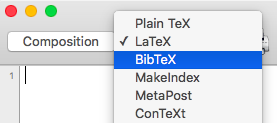
\includegraphics[height=2.2cm]{bibtex-texshop}
  \qquad
  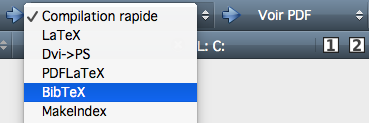
\includegraphics[height=2.2cm]{bibtex-texmaker}
  \caption{Interfaces de sélection du programme {\BibTeX} dans TeXShop
    (à gauche)
    et Texmaker (à droite)}
  \label{fig:bibliographie:editeurs}
\end{figure}

\begin{conseil}
  Aux toutes dernières étapes avant de rendre un document, s'assurer
  d'exécuter {\BibTeX} une dernière fois et de compiler avec
  pdf{\LaTeX} ou {\XeLaTeX} au moins deux fois. Le journal de la
  compilation (\emph{log file}) ne devrait pas rapporter de références
  manquantes (\emph{undefined references}).
\end{conseil}

1. citer (avec natbib)
2. construire la bibliographie avec BIBTeX
3. base de données
   - concepts de base et lien vers ressources complètes
   - style fr
4. conversion depuis Endnote

%%%
%%% Exercices
%%%

\section{Exercices}
\label{sec:bibliographie:exercices}

\Opensolutionfile{solutions}[solutions-bibliographie]

\begin{Filesave}{solutions}
\section*{Chapitre \ref*{chap:bibliographie}}
\addcontentsline{toc}{section}{Chapitre \protect\ref*{chap:bibliographie}}

\end{Filesave}

\Closesolutionfile{solutions}

%%% Local Variables:
%%% mode: latex
%%% TeX-engine: xetex
%%% TeX-master: "formation_latex-partie_2"
%%% coding: utf-8
%%% End:
